\section{Pasirinktos debesų kompiuterijos technologijos}

Šis skyrius žymi praktinės rašto darbo dalies pradžią, jame apžvelgiamos pasirinktos „Microsoft Azure“ debesų kompiuterijos tiekėjo paslaugos ir resursai argumentuojant pasirinkimo motyvus. „Azure“ platforma pasirinkta dėl autoriaus asmeninės patirties, tačiau rašto darbo autorius neabejoja dėl galimybės panašias paslaugas pasirinkti kitų tiekėjų, tokių kaip „Amazon AWS“ \footnote{AWS -- Amazon Web Services} ar „Google Cloud Platform“ platformose. \cite{MercedCloudBasedWebCrawler} moksliniame darbe, kuriuo šiame rašto darbe plačiai remiamasi kuriant peržiūros robotą, aprašyta sistema  buvo kurta pagal senąjį „Azure“ infrastruktūros modelį, kuris šiuo metu aktyviai nebepalaikomas, todėl įgyvendinant šį prototipą buvo pasitelkti naujesni „Azure“ debesų kompiuterijos tiekėjo įrankiai, kurie leistų užtikrinti analogišką aprašytos architektūros įgyvendinimą.

\subsection{Sistemos orchestravimas}

Įgyvendinant detalųjį architektūrinį saityno peržvalgos roboto sistemos dizainą ir renkantis iš technologijų, buvo pasirinkta „Microsoft Azure Service Fabric“ mikroservisų orchestravimo platforma, kuri apibrėžia ne tik sistemų klasterių valdymą ir išplėtimą, tačiau taip pat turi savo vykdomąją aplinką (angl. -- \textit{Service Fabric Runtime Environment}), kuri palaiko „Service Fabric“ programavimo modelius \cite{ServiceFabricTerminology}. Alternatyvi galimybė buvo rinktis „Azure Kubernetes Service“ orchestratoriaus paslaugą, tačiau „Service Fabric“ buvo pasirinktas dėl didelių vykdomosios aplinkos ir programavimo modelių galimybių, kurios suteikia daug abstrakcijos programuotojams -- leidžia orientuotis į verslo kodo rašymą paliekant infrastruktūrines surišimo problemas pačiai platformai.

\subsubsection{„Service Fabric“ infrastruktūra}

Šios platformos infrastruktūros konceptą apibrėžia 3 pagrindiniai komponentai \cite{ServiceFabricTerminology}:
\begin{itemize}
    \item Klasteris (angl. -- \textit{Cluster}) -- tinklu sujungtas išplečiamas rinkinys virtualių ar fizinių mašinų, kuriose diegiami „Service Fabric“ programų paketai, gali turėti kelis priskirtus mazgo tipus
    \item Mazgo tipas (angl. -- \textit{Node Type}) -- komponentas, kuris sujungia „Service Fabric“ klasterį su „Azure“ virtualių mašinų rinkiniu. Gali turėti ne daugiau nei vieną priskirtą virtualių mašinų rinkinį
    \item Virtualių mašinų išplėtimo rinkinys (angl. -- \textit{Virtual Machine Scale Set}) -- virtualių mašinų kolekcija, kurioje galima pridėti/trinti mašinas
    \item Mazgas (angl. -- \textit{Node}) -- virtuali arba fizinė mašina, kuri yra sudedamoji klasterio dalis, turi priskiriamą vardą
\end{itemize}

\ref{fig:sf_infrastructure} paveikslėlyje matomas infrastruktūros komponentų išsidėstymas. Vienas mazgo tipas visada būna pirminis, o kiti -- antriniai. Nerekomenduojama keisti pirminio mazgo tipo virtualių mašinų korekcijos virtualias mašinas jau paleidus klasterį, nes pakeitimas gali turėti neigiamos įtakos sklandžiam klasterio veikimui. Rašto darbe prototipas sudiegtas į vieno mazgo tipo klasterį, tai leido sutaupyti kaštų -- ši paslauga nerekomenduojama produkcinėms aplinoms, tačiau skirta testavimo tikslams.

\begin{figure}[htp!]
\centering
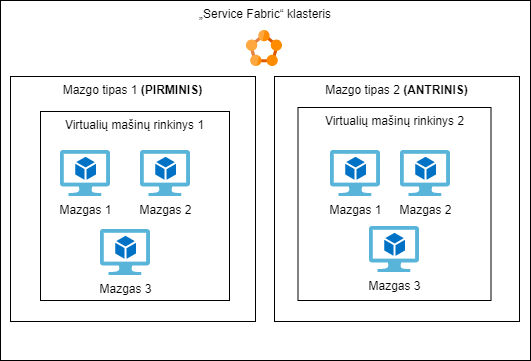
\includegraphics[scale=0.7]{img/SF_infrastructure.png}
\caption{„Service Fabric“ infrastruktūra \cite{ServiceFabricTerminology}}
\label{fig:sf_infrastructure}
\end{figure}

„Azure Service Fabric“ infrastruktūra palaiko tiek „Windows“, tiek „Linux“ operacines sistemas, rašto darbe naudojamas „Windows“ klasteris, kuris reikalauja daugiau minimalių sistemos resursų. Minimalūs rekomenduojami reikalavimai „Windows“ klasteriui yra šie:
\begin{itemize}
    \item 3,5 GB RAM operatyviosios atminties
    \item 50 GB SSD laikinos disko vietos
    \item 1 vienetas 2.4 GHz Intel Xeon vCPU procesorius
\end{itemize}
\subsubsection{„Service Fabric“ programavimo modelis}

„Service Fabric“ programavimo modelį sudaro šie pagrindiniai komponentai \cite{ServiceFabricTerminology}:

\begin{itemize}
    \item Programa (angl. -- \textit{Application}) -- rinkinys savarankiškų tarnybų (angl. -- \textit{Services}), kurios atlieka tam tikrą funkciją sistemoje
    \item Tarnyba (angl. -- \textit{Service}) -- tam tikros funkcijos atlikimo vienetas, mikroservisų architektūros vienetas
    \item Skaidinys (angl. -- \textit{Partition}) -- tarnybos duomenų skaidymo loginis vienetas, šiame rašto darbo prototipe nenaudojamas, todėl plačiau neaptariamas
    \item Kopija (angl. -- \textit{Replica}) -- duomenų kopijos, naudojamos tarnybose su būsena (angl. -- \textit{stateful services}), šio rašto darbo prototipo įgyvendinime nenaudojamos
\end{itemize}

\begin{figure}[htp!]
\centering
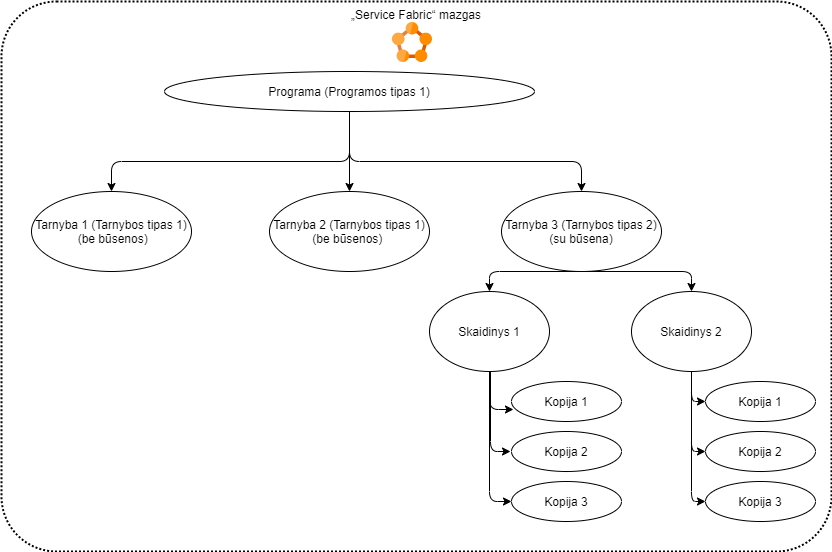
\includegraphics[scale=0.5]{img/SF_programming_model.png}
\caption{„Service Fabric“ programavimo modelis \cite{ServiceFabricTerminology}}
\label{fig:sf_programming_model}
\end{figure}

„Azure Service Fabric“ programavimo modelis apibrėžia 4 tipų tarnybas:
\begin{enumerate}
    \item Tarnybos be būsenos (angl. -- \textit{Stateless services}) -- tarnybos, kurios operatyvioje atmintyje nesaugo ir nenaudoja duomenų, visi duomenys išoriniai -- gali būti SQL duombazė ar NoSQL talpykla \cite{ServiceFabricTerminology}
    \item Tarnybos su būsena (angl. -- \textit{Stateful services}) -- tarnybos, kurios turi savo priskirtus duomenis ir būseną, kuri yra replikuojama tarp skirtingų mazgų klasteryje \cite{ServiceFabricTerminology}
    \item Išorinio kodo tarnybas (angl. -- \textit{Guest executables}) -- klateryje galima paleisti tarnybas, kurios vykdo išorinį vykdomąjį failą (.exe failą), kuris sukurtas visiškai kitomis programavimo kalbomis, nei vykdomoji „Service Fabric“ aplinka \cite{ServiceFabricTerminology}
    \item Konteinerių tarnybas (angl. -- \textit{Container services}) -- tarnybos paketą galima talpinti virtualiame konteineryje (pvz.: „Docker“), kuriame taip pat izoliuota „Service Fabric“ vykdomoji aplinka ir visos reikalingos priklausomos bibliotekos \cite{ServiceFabricTerminology} 
\end{enumerate}

Šiame rašto darbe peržiūros agentai įgyvendinti kaip tarnybos be būsenos, nes visa jiems reikalinga informacija saugoma arba eilėse, arba SQL/NoSQL duombazėse, todėl vidinės būsenos mechanizmai, kuriuos siūlo „Service Fabric“ modelis, nereikalingi.

\subsection{Virtualių mašinų rinkiniai}

„Service Fabric“ klasteris turi priskiriamus vieną arba daugiau virtualių mašinų rinkinius (angl. -- \textit{„Virtual Machine Scale Sets“}), kurie leidžia logiškai grupuoti daug virtualių mašinų, kurias galima valdyti centralizuotai -- diegti atnaujinimus, keisti konfigūracija. \cite{VirtualMachineScaleSets}. Visos virtualios mašinos rinkinyje yra sukuriamos iš bendro operacinės sistemos atvaizdžio (angl. -- \textit{OS image}). \cite{VirtualMachineScaleSets}.

Kuriant virtualių mašinų išplėtimo rinkinį, automatiškai sukuriamas ir apkrovos išlyginimo (angl. -- \textit{load balancing}) resursas, kuris leidžia reaguoti į virtualių mašinų apkrovų duomenis ir tolygiai paskirstyti srautą. \cite{VirtualMachineScaleSets}. Taip pat sukuriamas virtualus tinklas, kuris leidžia rinkinyje esančioms virtualioms mašinoms bendrauti vienai su kita.

Įgyvendinant šio rašto darbo prototipą naudojamas klasteris su vienu virtualių mašinų išplėtimo rinkiniu, kuriame sudiegta viena virtuali mašina.

\pagebreak

\subsection{Eilių mechanizmas}

Įgyvendinant išskaidytą peržvalgos robotą, asinchroninę komunikaciją tarp atskirų sistemos komponentų užtikrina eilių mechanizmas, veikiantis FIFO\footnote{First-In-First-Out} principu. „Azure“ paslaugų modelis siūlo 2 skirtingus eilių sprendimus:
\begin{itemize}
    \item „Service Bus Queues“ -- „Azure Storage“ paslaugų infrastruktūros dalis, paprasta REST programinė sąsaja \cite{QueuesStorageVsServiceBus}
    \item „Storage Queues“ -- „Azure messaging“ infrastruktūros dalis, specializuotai skirta sistemų integracijos šablonų įgyvendinimui (pvz.: -- „publish-subscribe“) modelis \cite{QueuesStorageVsServiceBus}
\end{itemize}

Platesnis šių sprendimų palyginimas matomas lentelėje.

% Table generated by Excel2LaTeX from sheet 'crawling_vs_scraping'
\begin{table}[htbp]
  \centering
  \caption{„Storage Queues“ ir „Service Bus Queues“ palyginimas \cite{QueuesStorageVsServiceBus}}
    \begin{tabular}{|l|l|l|}
    \hline
    \textbf{Aspektas} & \textbf{„Azure Storage Queues“} & \textbf{„Azure Service Bus Queues“} \bigstrut\\
    \hline
    Atsiradimo laikas & Atsirado anksčiau & Pristatyta vėliau, 2014 metais \\
    \hline
    Eilės talpa & 1 TB ir daugiau & <= 80GB \\
    \hline
    FIFO užtikrinimas & Negarantuotas & Garantuotas \\
    \hline
    „Long-polling“ palaikymas & Nepalaikoma & Palaikoma \\
    \hline
    „AMQP 1.0“ standartas & Nepalaikomas & Palaikomas \\
    \hline
    Automatinis „dead-letter“ mechanizmas & Nepalaikomas & Palaikomas \\
    \hline
    Eilių skaičius & Neribojamas & 10000 \\
    \hline
    \end{tabular}%
  \label{tab:agent_registry_table}%
\end{table}%

Įgyvendinant prototipą rašto darbo autoriaus sprendimu pasirinkta „Azure Service Bus Queues“ technologija dėl šių esminių priežasčių:

\begin{enumerate}
    \item Palaikoma „long-polling“ technologija -- kuriant „Service Fabric“ tarnybas ir jų klausytojus (angl. -- \textit{service listeners}) nenorėta cikle naudoti HTTP „polling“ metodo, kuris lemtų sudėtingesnės kodo infrastruktūros poreikį
    \item FIFO palaikymas -- norima, kad pirmiau aptikti puslapiai būtų atitinkamai žvalgomi greičiau
    \item Rasta biblioteka, kuri užtikrino „Service Fabric“ ir „Service Bus“ paslaugų integraciją be papildomo kodo rašymo\footnote{Service Fabric Service Bus -- https://github.com/loekd/ServiceFabric.ServiceBus}
\end{enumerate}

\subsubsection{Pasirinktos technologijos rizikos}

\cite{MercedCloudBasedWebCrawler} siūlytoje architektūroje buvo naudojama „Azure Storage Queues“ paslauga, pagrindinės rizikos, kurios gali kilti naudojant rašto darbo autoriaus pasirinktą technologiją yra susijusios su apribotu plečiamumu, nes „Service Bus“ nepalaiko daugiau nei 10000 eilių, o šiame roboto prototipe kiekvienas domenas turi dinamiškai sukuriamą agento eilę. Taip pat apribotas eilės dydis (80GB), nes platus žvalgymas apima dešimtis milijonų puslapių.

\subsection{Reliacinė duombazė}

Vienas iš prototipo komponentų -- agentų registras -- realizuotas panaudojant griežtą schemą palaikančios „Microsoft SQL Server“ reliacinės duomenų bazės atitikmenį „Azure“ platformoje, kuris veikia PaaS\footnote{Platform-as-a-service} principu -- „Azure SQL“ duomenų bazės serverį. Ši debesų kompiuterijos paslauga leidžia kontroliuoti ugniasienės nustatymus, kad tik tam tikrų IP adresų klientai galėtų komunikuoti su duomenų baze, todėl įgyvendinant prototipą, virtualių mašinų kolekcijos virtualus tinklas buvo pridėtas kaip SQL duomenų bazės ugniasienės taisyklė. Platforma taip pat palaiko automatinį resursų išplečiamumą, kuris gali būti vykdomas reaguojant į naudojimo apkrovų statistiką.

\subsubsection{Duombazės pajėgumo metrika}

Kuriant „Azure SQL“ serverį svarbu atsižvelgti, kokio galingumo duombazės serverio sistemai reikia. Kadangi ši paslauga veikia PaaS principu, duombazės serverio pajėgumas nėra nustatomas tradicine procesoriaus branduolių, operatyviosios atminties ir disko talpos kombinacija. Vietoje to naudojama abstraktesnė metrika, pavadinimu „Data Trancation Unit“ (toliau -- DTU) \cite{DTUMetric}.

DTU apibrėžimas pagal „Microsoft“ dokumentaciją -- maišyta procesoriaus, operatyviosios atminties, duomenų ir tranzakcijų įrašų I/O skaičiaus metrika. \cite{DTUMetric} Dvigubinant DTU skaičių atitikamai dvigubinamas duomenų bazei priskiriamų resursų pajėgumas.

\subsection{NoSQL saugykla}

Pastovus aplankytų URL adresų sąrašas, taip pat svetainių Javascript atvaizdavimo analizavimo kontrolinės sumos saugomos „Azure Table Storage“ NoSQL duomenų bazėje. Ši paslauga yra „Key-value“ tipo NoSQL duombazės tipo. 

Tokio tipo duomenų bazės yra tam tikra prasme maišos lentelės (angl. -- \textit{hash tables}) ir pasižymi \cite{KeyValueStores}:
\begin{itemize}
    \item Itin greitos užklausos pagal rakto reikšmę (ieškoti pagal reikšmę nėra efektyvu, lyginant su reliacinėmis duomenų bazėmis ir jų WHERE sakinių konstruktais)
    \item Nėra duomenų bazės schemos, todėl lengva prisitaikyti prie evoliucionuojančių sistemų ir duomenų
    \item Lengvą išplėsti tokios duomenų bazės talpą pagal poreikius, nes duomenys paskirstomi skirtinguose fiziniuose mazguose, sujungtuose tinklu
    \item Nepalaiko sudėtingų paieškos operacijų, reikalaujančių duomenų apjungimo, išorinių raktų ar duombazės procedūrų
\end{itemize}

\pagebreak

\subsubsection{„Azure Storage Table“ modelis}

Šios paslaugos esmę apibrėžia 4 pagrindiniai elementai \cite{TableStorageModel}:
\begin{itemize}
    \item \textit{„Storage“ paskyra} -- unikalus resurso savininko indentifikavimo ir autorizavimo mechanizmas
    \item \textit{Lentelė} -- paskyroje esantis obektų rinkinys, neturintis griežtos atributų schemos
    \item \textit{Esybė} -- atributų rinkinys, panašus į reliacinių duomenų bazių eilutę
    \item \textit{Atributas} -- (angl. -- \textit{properties}) rakto-reikšmės pora, nusakanti esybės konkretų požymį
\end{itemize}

Šių esybių sąryšis pavaizduotas \ref{fig:storage_table_model} paveikslėlyje:

\begin{figure}[htp!]
\hspace{-1cm}
\centering
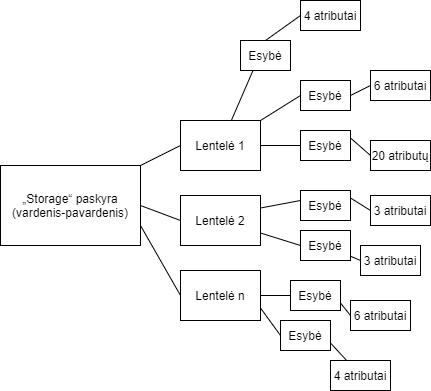
\includegraphics[scale=0.5]{img/Storage_modelis.png}
\caption{„Storage Table“ modelis}
\label{fig:storage_table_model}
\end{figure}

Aprašytos paslaugos modelyje esybė palaiko daugiausiai iki 255 atributų, iš kurių 3 yra sisteminiai ir privalomi: \cite{TableStorageModel}

\begin{itemize}
    \item \textit{PartitionKey} -- pirmoji sudėtinė pirminio rakto dalis, skaidinys, kuris leidžia skaidyti saugyklos duomenis topologiškai skirtinguose mazguose ir lemia didelį tokių duomenų bazių išplečiamumą
    \item \textit{RowKey} -- antroji sudėtinė pirminio rakto dalis, turi būti unikali kiekviename skaidinyje
    \item \textit{Timestamp} -- paskutinė esybės koregavimo data ir laikas
\end{itemize}

\begin{figure}[htp!]
\hspace{-1cm}
\centering
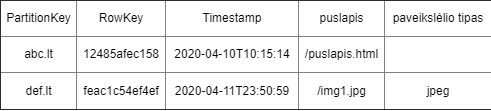
\includegraphics[scale=0.7]{img/Storage_table.png}
\caption{„Storage Table“ lentelės struktūra \cite{TableStorageModel}}
\label{fig:storage_table_structure}
\end{figure}

Kaip matome iš \ref{fig:storage_table_structure} lentelės, esybių atributų skaičius lentelėje gali skirtis, nes nėra apibrėžtos schemos.